
\end{figure}
\usetikzlibrary{arrows,automata}
\begin{figure}

\begin{tabular}{ ccc  }
\subfigure[Initial Event]{

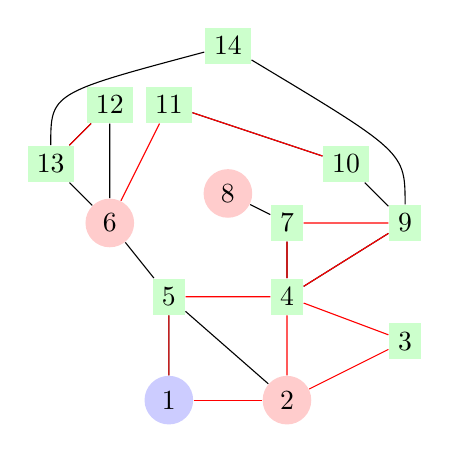
\begin{tikzpicture}[scale=.75]

\node[circle,fill=blue!20] (one) at (3,0) {1};
\node[circle,fill=red!20] (two) at (5,0) {2};
\node[rectangle,fill=green!20] (three) at (7,1) {3};
\node[rectangle,fill=green!20] (four) at (5,1.75) {4};
\node[rectangle,fill=green!20] (five) at (3,1.75) {5};
\node[circle,fill=red!20] (six) at (2,3) {6};
\node[rectangle,fill=green!20] (seven) at (5,3) {7};
\node[circle,fill=red!20] (eight) at (4,3.5) {8};
\node[rectangle,fill=green!20] (nine) at (7,3) {9};
\node[rectangle,fill=green!20] (ten) at (6,4) {10};
\node[rectangle,fill=green!20] (eleven) at (3,5) {11};
\node[rectangle,fill=green!20] (twelve) at (2,5) {12};
\node[rectangle,fill=green!20] (thirteen) at (1,4) {13};
\node[rectangle,fill=green!20] (fourteen) at (4,6) {14};


\draw[red] (one) -- (two) ;
\draw (one) -- (five);
\draw[red] (one) -- (five) ; 
\draw[red] (two) -- (three) ; 
\draw[red] (two) -- (four) ; 
\draw (two) -- (five) ; 
\draw[red] (three) -- (four) ; 
\draw[red] (four) -- (five) ; 
\draw (four) -- (seven);
\draw[red] (four) -- (seven) ;
\draw (four) -- (nine);
\draw[red] (four) -- (nine) ; 
\draw (five) -- (six) ; 
\draw[red] (six) -- (eleven) ; 
\draw (six) -- (twelve) ; 
\draw (six) -- (thirteen) ; 
\draw (seven) -- (eight) ; 
\draw[red] (seven) -- (nine) ; 
\draw (nine) -- (ten) ; 
\draw (nine) .. controls +(up:1.2cm) .. (fourteen) ;
\draw (ten) -- (eleven);
\draw[red] (ten) -- (eleven) ;  
\draw (twelve) -- (thirteen);
 \draw[red](twelve) -- (thirteen) ; 
\draw (thirteen) .. controls +(up:1.2cm) .. (fourteen) ; 
\end{tikzpicture}
} &
\subfigure[Stage 1]{
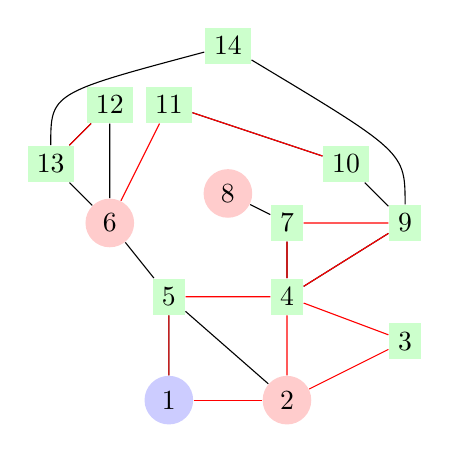
\begin{tikzpicture}[scale=.75]

\node[circle,fill=blue!20] (one) at (3,0) {1};
\node[circle,fill=red!20] (two) at (5,0) {2};
\node[rectangle,fill=green!20] (three) at (7,1) {3};
\node[rectangle,fill=green!20] (four) at (5,1.75) {4};
\node[rectangle,fill=green!20] (five) at (3,1.75) {5};
\node[circle,fill=red!20] (six) at (2,3) {6};
\node[rectangle,fill=green!20] (seven) at (5,3) {7};
\node[circle,fill=red!20] (eight) at (4,3.5) {8};
\node[rectangle,fill=green!20] (nine) at (7,3) {9};
\node[rectangle,fill=green!20] (ten) at (6,4) {10};
\node[rectangle,fill=green!20] (eleven) at (3,5) {11};
\node[rectangle,fill=green!20] (twelve) at (2,5) {12};
\node[rectangle,fill=green!20] (thirteen) at (1,4) {13};
\node[rectangle,fill=green!20] (fourteen) at (4,6) {14};


\draw[red] (one) -- (two) ;
\draw (one) -- (five);
\draw[red] (one) -- (five) ; 
\draw[red] (two) -- (three) ; 
\draw[red] (two) -- (four) ; 
\draw (two) -- (five) ; 
\draw[red] (three) -- (four) ; 
\draw[red] (four) -- (five) ; 
\draw (four) -- (seven);
\draw[red] (four) -- (seven) ;
\draw (four) -- (nine);
\draw[red] (four) -- (nine) ; 
\draw (five) -- (six) ; 
\draw[red] (six) -- (eleven) ; 
\draw (six) -- (twelve) ; 
\draw (six) -- (thirteen) ; 
\draw (seven) -- (eight) ; 
\draw[red] (seven) -- (nine) ; 
\draw (nine) -- (ten) ; 
\draw (nine) .. controls +(up:1.2cm) .. (fourteen) ;
\draw (ten) -- (eleven);
\draw[red] (ten) -- (eleven) ;  
\draw (twelve) -- (thirteen);
 \draw[red](twelve) -- (thirteen) ; 
\draw (thirteen) .. controls +(up:1.2cm) .. (fourteen) ; 
\end{tikzpicture}
}					&
\subfigure[Stage 2]{
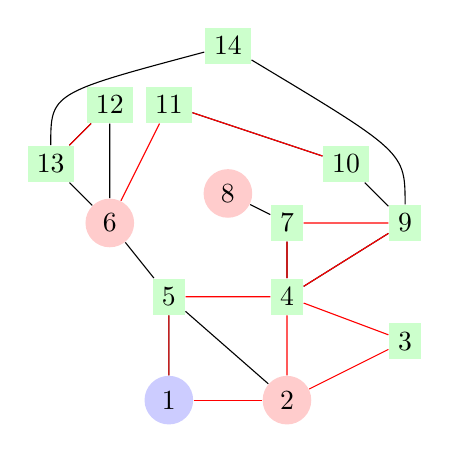
\begin{tikzpicture}[scale=.75]

\node[circle,fill=blue!20] (one) at (3,0) {1};
\node[circle,fill=red!20] (two) at (5,0) {2};
\node[rectangle,fill=green!20] (three) at (7,1) {3};
\node[rectangle,fill=green!20] (four) at (5,1.75) {4};
\node[rectangle,fill=green!20] (five) at (3,1.75) {5};
\node[circle,fill=red!20] (six) at (2,3) {6};
\node[rectangle,fill=green!20] (seven) at (5,3) {7};
\node[circle,fill=red!20] (eight) at (4,3.5) {8};
\node[rectangle,fill=green!20] (nine) at (7,3) {9};
\node[rectangle,fill=green!20] (ten) at (6,4) {10};
\node[rectangle,fill=green!20] (eleven) at (3,5) {11};
\node[rectangle,fill=green!20] (twelve) at (2,5) {12};
\node[rectangle,fill=green!20] (thirteen) at (1,4) {13};
\node[rectangle,fill=green!20] (fourteen) at (4,6) {14};


\draw[red] (one) -- (two) ;
\draw (one) -- (five);
\draw[red] (one) -- (five) ; 
\draw[red] (two) -- (three) ; 
\draw[red] (two) -- (four) ; 
\draw (two) -- (five) ; 
\draw[red] (three) -- (four) ; 
\draw[red] (four) -- (five) ; 
\draw (four) -- (seven);
\draw[red] (four) -- (seven) ;
\draw (four) -- (nine);
\draw[red] (four) -- (nine) ; 
\draw (five) -- (six) ; 
\draw[red] (six) -- (eleven) ; 
\draw (six) -- (twelve) ; 
\draw (six) -- (thirteen) ; 
\draw (seven) -- (eight) ; 
\draw[red] (seven) -- (nine) ; 
\draw (nine) -- (ten) ; 
\draw (nine) .. controls +(up:1.2cm) .. (fourteen) ;
\draw (ten) -- (eleven);
\draw[red] (ten) -- (eleven) ;  
\draw (twelve) -- (thirteen);
 \draw[red](twelve) -- (thirteen) ; 
\draw (thirteen) .. controls +(up:1.2cm) .. (fourteen) ; 
\end{tikzpicture}
}				\\

\subfigure[Stage 3]{
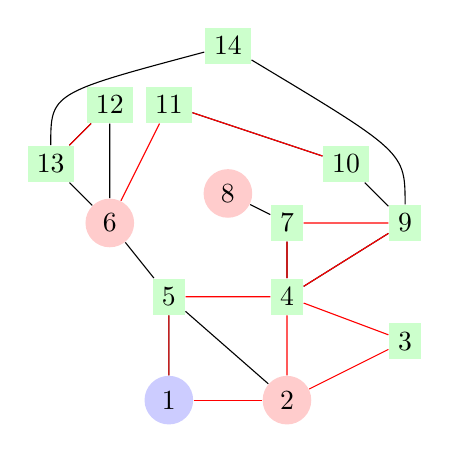
\begin{tikzpicture}[scale=.75]

\node[circle,fill=blue!20] (one) at (3,0) {1};
\node[circle,fill=red!20] (two) at (5,0) {2};
\node[rectangle,fill=green!20] (three) at (7,1) {3};
\node[rectangle,fill=green!20] (four) at (5,1.75) {4};
\node[rectangle,fill=green!20] (five) at (3,1.75) {5};
\node[circle,fill=red!20] (six) at (2,3) {6};
\node[rectangle,fill=green!20] (seven) at (5,3) {7};
\node[circle,fill=red!20] (eight) at (4,3.5) {8};
\node[rectangle,fill=green!20] (nine) at (7,3) {9};
\node[rectangle,fill=green!20] (ten) at (6,4) {10};
\node[rectangle,fill=green!20] (eleven) at (3,5) {11};
\node[rectangle,fill=green!20] (twelve) at (2,5) {12};
\node[rectangle,fill=green!20] (thirteen) at (1,4) {13};
\node[rectangle,fill=green!20] (fourteen) at (4,6) {14};


\draw[red] (one) -- (two) ;
\draw (one) -- (five);
\draw[red] (one) -- (five) ; 
\draw[red] (two) -- (three) ; 
\draw[red] (two) -- (four) ; 
\draw (two) -- (five) ; 
\draw[red] (three) -- (four) ; 
\draw[red] (four) -- (five) ; 
\draw (four) -- (seven);
\draw[red] (four) -- (seven) ;
\draw (four) -- (nine);
\draw[red] (four) -- (nine) ; 
\draw (five) -- (six) ; 
\draw[red] (six) -- (eleven) ; 
\draw (six) -- (twelve) ; 
\draw (six) -- (thirteen) ; 
\draw (seven) -- (eight) ; 
\draw[red] (seven) -- (nine) ; 
\draw (nine) -- (ten) ; 
\draw (nine) .. controls +(up:1.2cm) .. (fourteen) ;
\draw (ten) -- (eleven);
\draw[red] (ten) -- (eleven) ;  
\draw (twelve) -- (thirteen);
 \draw[red](twelve) -- (thirteen) ; 
\draw (thirteen) .. controls +(up:1.2cm) .. (fourteen) ; 
\end{tikzpicture}
}					&

\subfigure[Stage 4]{
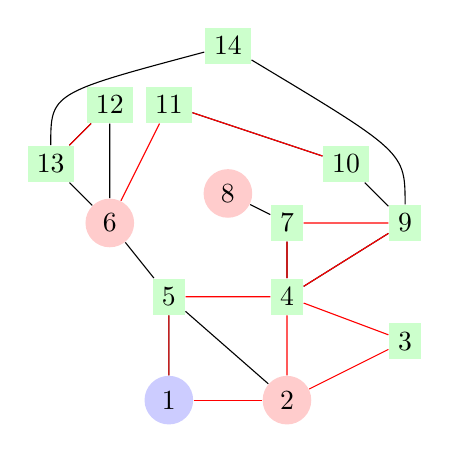
\begin{tikzpicture}[scale=.75]

\node[circle,fill=blue!20] (one) at (3,0) {1};
\node[circle,fill=red!20] (two) at (5,0) {2};
\node[rectangle,fill=green!20] (three) at (7,1) {3};
\node[rectangle,fill=green!20] (four) at (5,1.75) {4};
\node[rectangle,fill=green!20] (five) at (3,1.75) {5};
\node[circle,fill=red!20] (six) at (2,3) {6};
\node[rectangle,fill=green!20] (seven) at (5,3) {7};
\node[circle,fill=red!20] (eight) at (4,3.5) {8};
\node[rectangle,fill=green!20] (nine) at (7,3) {9};
\node[rectangle,fill=green!20] (ten) at (6,4) {10};
\node[rectangle,fill=green!20] (eleven) at (3,5) {11};
\node[rectangle,fill=green!20] (twelve) at (2,5) {12};
\node[rectangle,fill=green!20] (thirteen) at (1,4) {13};
\node[rectangle,fill=green!20] (fourteen) at (4,6) {14};


\draw[red] (one) -- (two) ;
\draw (one) -- (five);
\draw[red] (one) -- (five) ; 
\draw[red] (two) -- (three) ; 
\draw[red] (two) -- (four) ; 
\draw (two) -- (five) ; 
\draw[red] (three) -- (four) ; 
\draw[red] (four) -- (five) ; 
\draw (four) -- (seven);
\draw[red] (four) -- (seven) ;
\draw (four) -- (nine);
\draw[red] (four) -- (nine) ; 
\draw (five) -- (six) ; 
\draw[red] (six) -- (eleven) ; 
\draw (six) -- (twelve) ; 
\draw (six) -- (thirteen) ; 
\draw (seven) -- (eight) ; 
\draw[red] (seven) -- (nine) ; 
\draw (nine) -- (ten) ; 
\draw (nine) .. controls +(up:1.2cm) .. (fourteen) ;
\draw (ten) -- (eleven);
\draw[red] (ten) -- (eleven) ;  
\draw (twelve) -- (thirteen);
 \draw[red](twelve) -- (thirteen) ; 
\draw (thirteen) .. controls +(up:1.2cm) .. (fourteen) ; 
\end{tikzpicture}
}					&

\subfigure[Stage 5]{
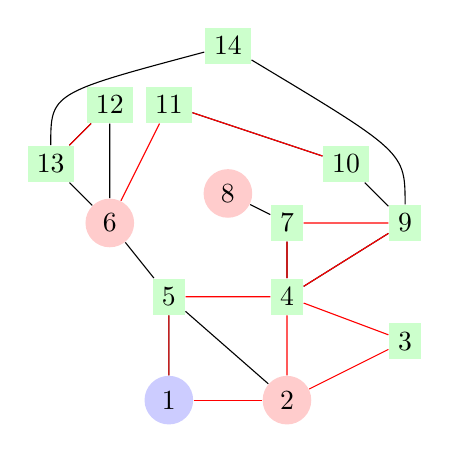
\begin{tikzpicture}[scale=.75]

\node[circle,fill=blue!20] (one) at (3,0) {1};
\node[circle,fill=red!20] (two) at (5,0) {2};
\node[rectangle,fill=green!20] (three) at (7,1) {3};
\node[rectangle,fill=green!20] (four) at (5,1.75) {4};
\node[rectangle,fill=green!20] (five) at (3,1.75) {5};
\node[circle,fill=red!20] (six) at (2,3) {6};
\node[rectangle,fill=green!20] (seven) at (5,3) {7};
\node[circle,fill=red!20] (eight) at (4,3.5) {8};
\node[rectangle,fill=green!20] (nine) at (7,3) {9};
\node[rectangle,fill=green!20] (ten) at (6,4) {10};
\node[rectangle,fill=green!20] (eleven) at (3,5) {11};
\node[rectangle,fill=green!20] (twelve) at (2,5) {12};
\node[rectangle,fill=green!20] (thirteen) at (1,4) {13};
\node[rectangle,fill=green!20] (fourteen) at (4,6) {14};


\draw[red] (one) -- (two) ;
\draw (one) -- (five);
\draw[red] (one) -- (five) ; 
\draw[red] (two) -- (three) ; 
\draw[red] (two) -- (four) ; 
\draw (two) -- (five) ; 
\draw[red] (three) -- (four) ; 
\draw[red] (four) -- (five) ; 
\draw (four) -- (seven);
\draw[red] (four) -- (seven) ;
\draw (four) -- (nine);
\draw[red] (four) -- (nine) ; 
\draw (five) -- (six) ; 
\draw[red] (six) -- (eleven) ; 
\draw (six) -- (twelve) ; 
\draw (six) -- (thirteen) ; 
\draw (seven) -- (eight) ; 
\draw[red] (seven) -- (nine) ; 
\draw (nine) -- (ten) ; 
\draw (nine) .. controls +(up:1.2cm) .. (fourteen) ;
\draw (ten) -- (eleven);
\draw[red] (ten) -- (eleven) ;  
\draw (twelve) -- (thirteen);
 \draw[red](twelve) -- (thirteen) ; 
\draw (thirteen) .. controls +(up:1.2cm) .. (fourteen) ; 
\end{tikzpicture}
}	
\end{tabular}
\caption{ \label{fig:cascade-example} An example of a cascading power failure }
\end{figure}
